\section{Additional Results}\label{additional_results}
\subsection{Kernel Density Estimate plots and Trace Plots}
Shown are the Kernel Density Estimate plots of Model 1 for each sampler. In addition, trace plots are shown for the scenario with 5 observations, because here the second mode is relatively pronounced. Trace plots show all 10 chains of the selected ensembles. For each sampler one ensemble was selected for the wide prior and one for the narrow prior, based on their $\hat{R}$, with the ensembles with the highest $\hat{R}$ being selected.  These KDE plots and trace plots for AI, DE and DE-SNK are given in Sections \ref{sub_AI}, \ref{sub_DE} and \ref{sub_DE-SNK}, respectively. Finally, pairs plots for AI and DE are given in \hyperref[sub_pairsplots]{\textcolor{blue}{Section }\ref{sub_pairsplots}}.

\newpage
\subsubsection{AI}\label{sub_AI}
\begin{figure*}[ht]
\centering
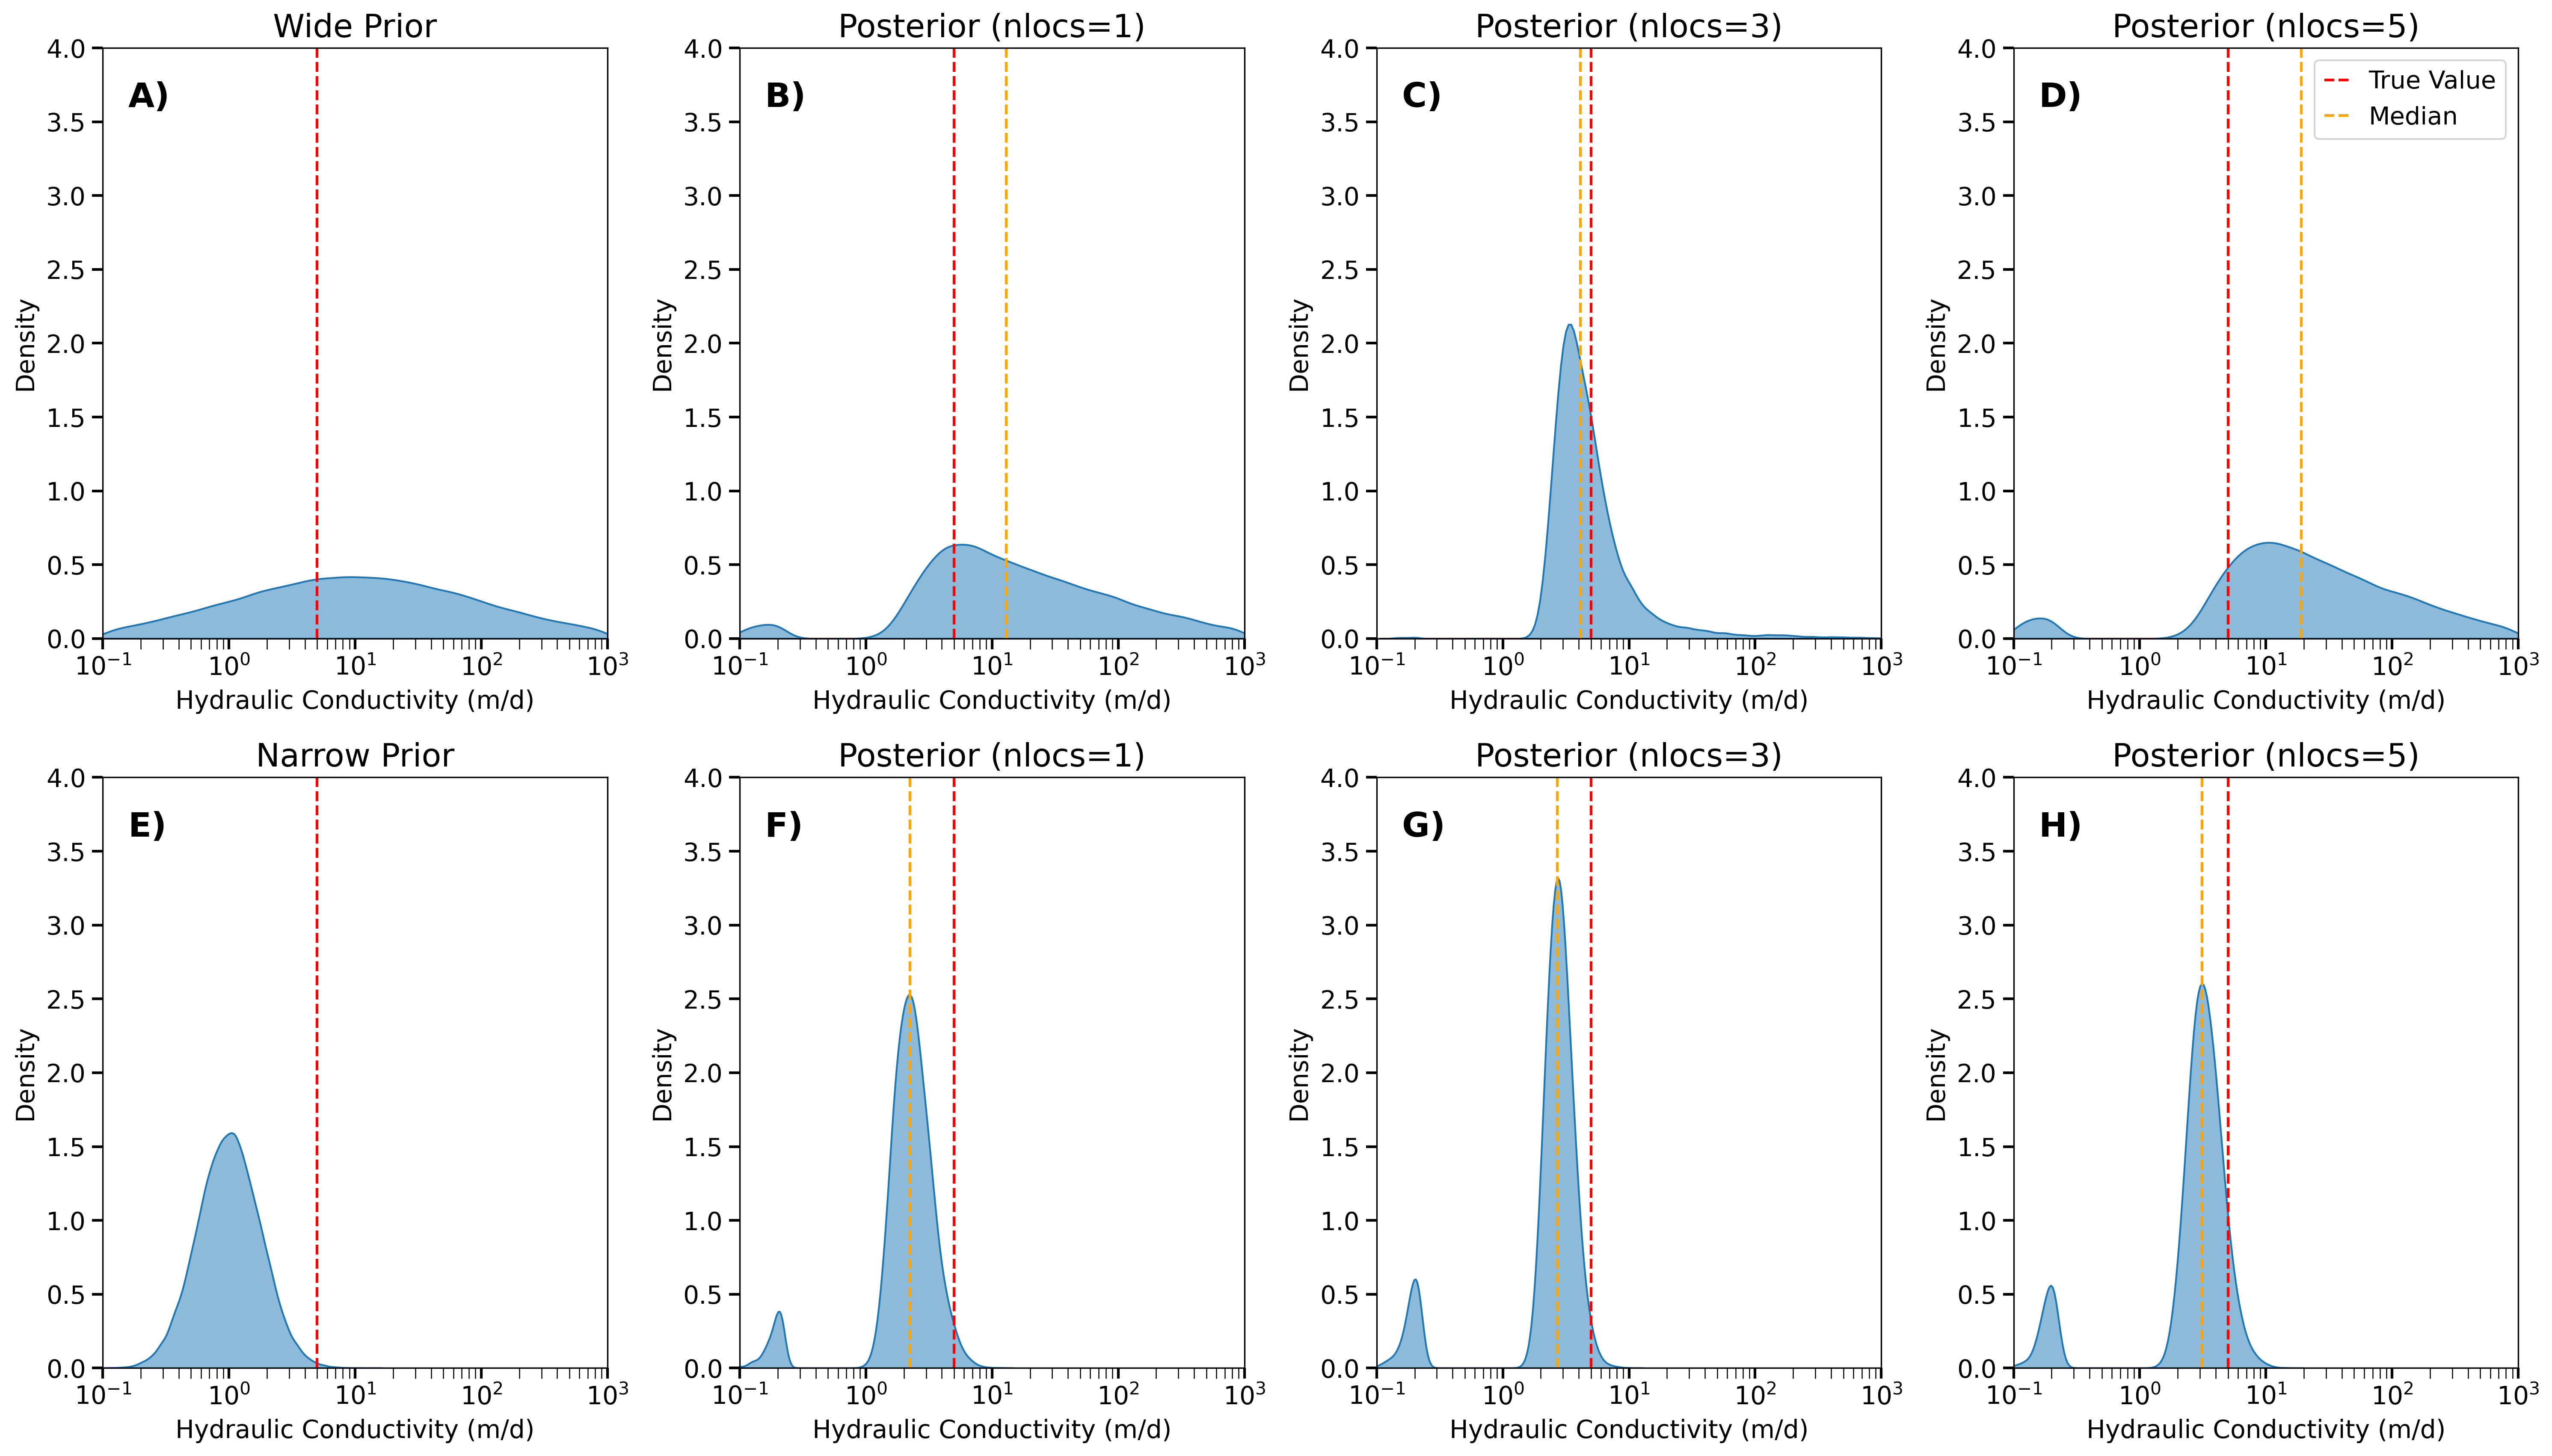
\includegraphics[width=1.0\textwidth]{Figures/appendix_figs/kde_model1_Stretch.png}
\caption{Kernel Density Estimate plots for the only parameter of Model 1 \textbf{($\theta_1$)}, which was calibrated with AI. \textbf{A)} shows the uninformative prior. \textbf{B), C)} and \textbf{D)} show the posteriors after calibrating $\theta_1$ with: the uninformative prior in combination with 1,3 or 5 observations for evaluating the likelihood. Similarly, \textbf{E)} shows the informative prior. \textbf{F), G)} and \textbf{H)} show the posteriors after calibrating $\theta_1$ with: the informative prior in combination with 1,3 or 5 observations for evaluating the likelihood. In each plot the dashed red line indicates the true value for $\theta_1$. Similarly, the posterior median is indicated by a dashed yellow line.}\label{fig_kde_model1_Stretch}
\end{figure*}


\begin{figure*}[ht]
\centering
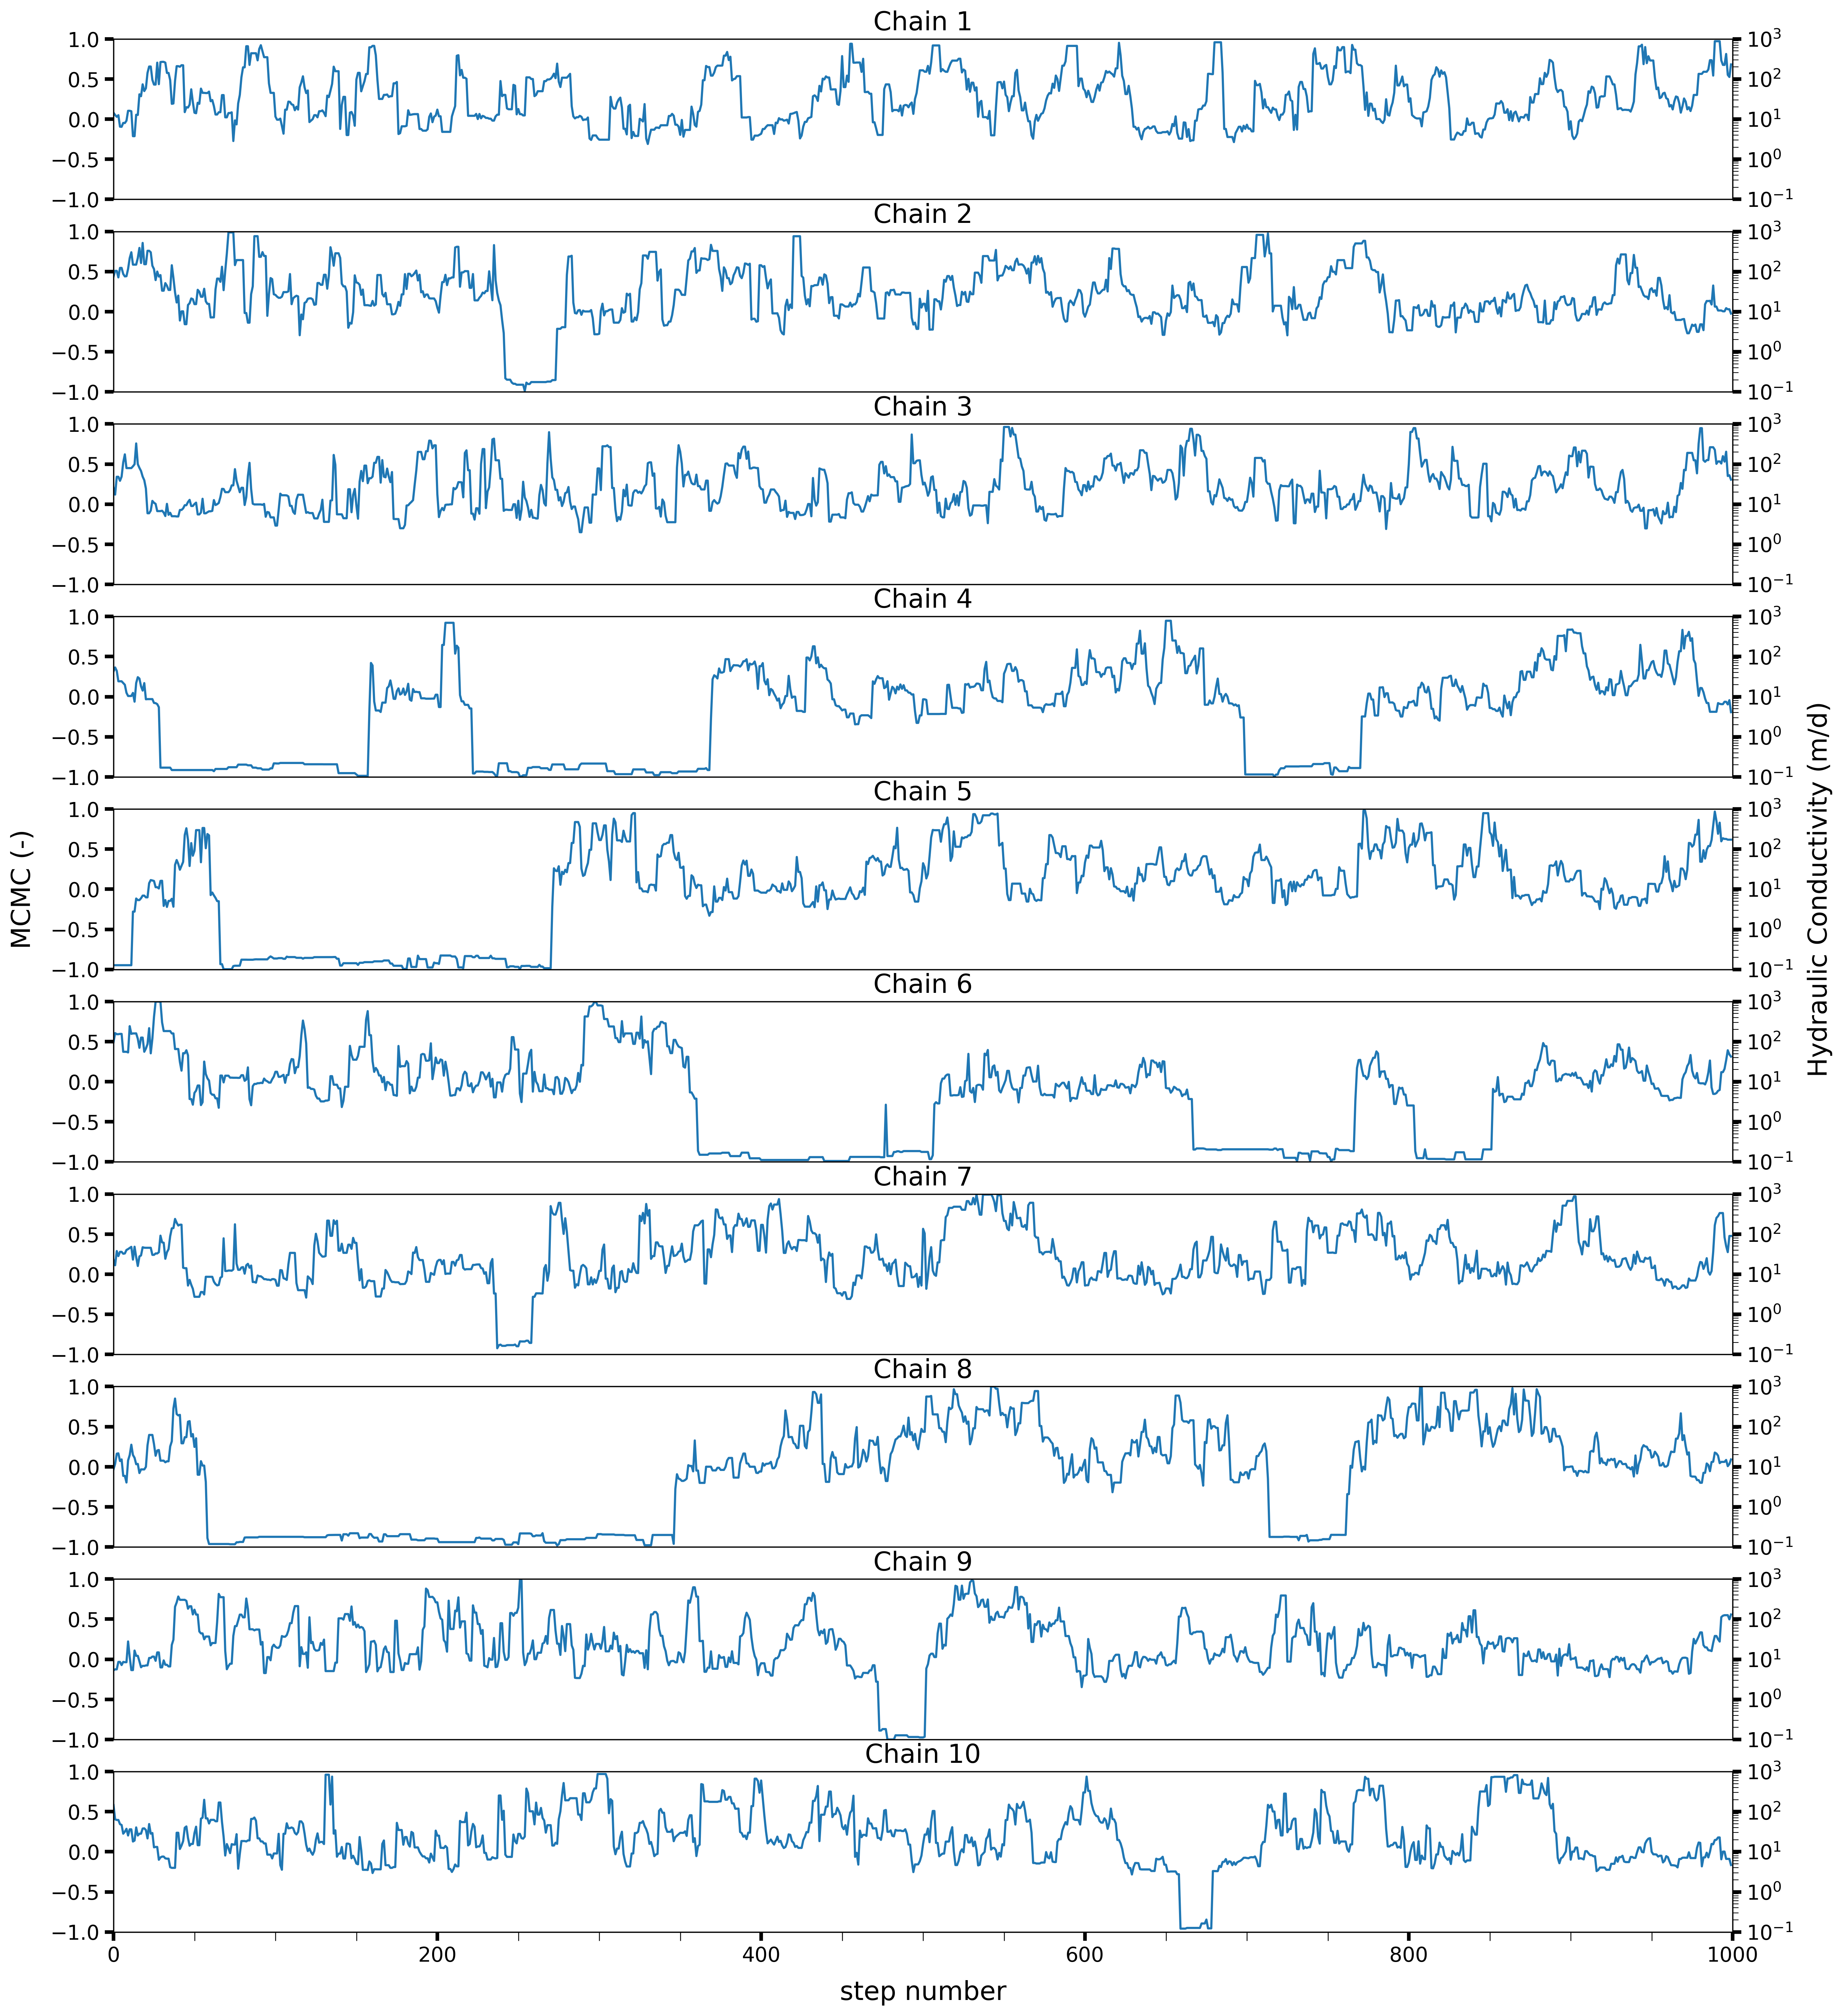
\includegraphics[width=1.0\textwidth]{Figures/appendix_figs/trace_plots_ensemble5_Stretch priorbroad.png}
\caption{Trace plots for ensemble 5 of AI, from calibrating  $\theta_1$ in Model 1 with the wide prior and 5 observations. All post burn-in steps are shown for all 10 chains, with the step number given on the x-axis. On the left y-axis the parameter values as used by the MCMC algorithm are shown. And on the right y-axis the transformed parameter values, used by MODFLOW 6, for calculation of the likelihood.  For this ensemble $\hat{R}=1.11$.}\label{traceplot_AI_priorbroad}
\end{figure*}

\begin{figure*}[ht]
\centering
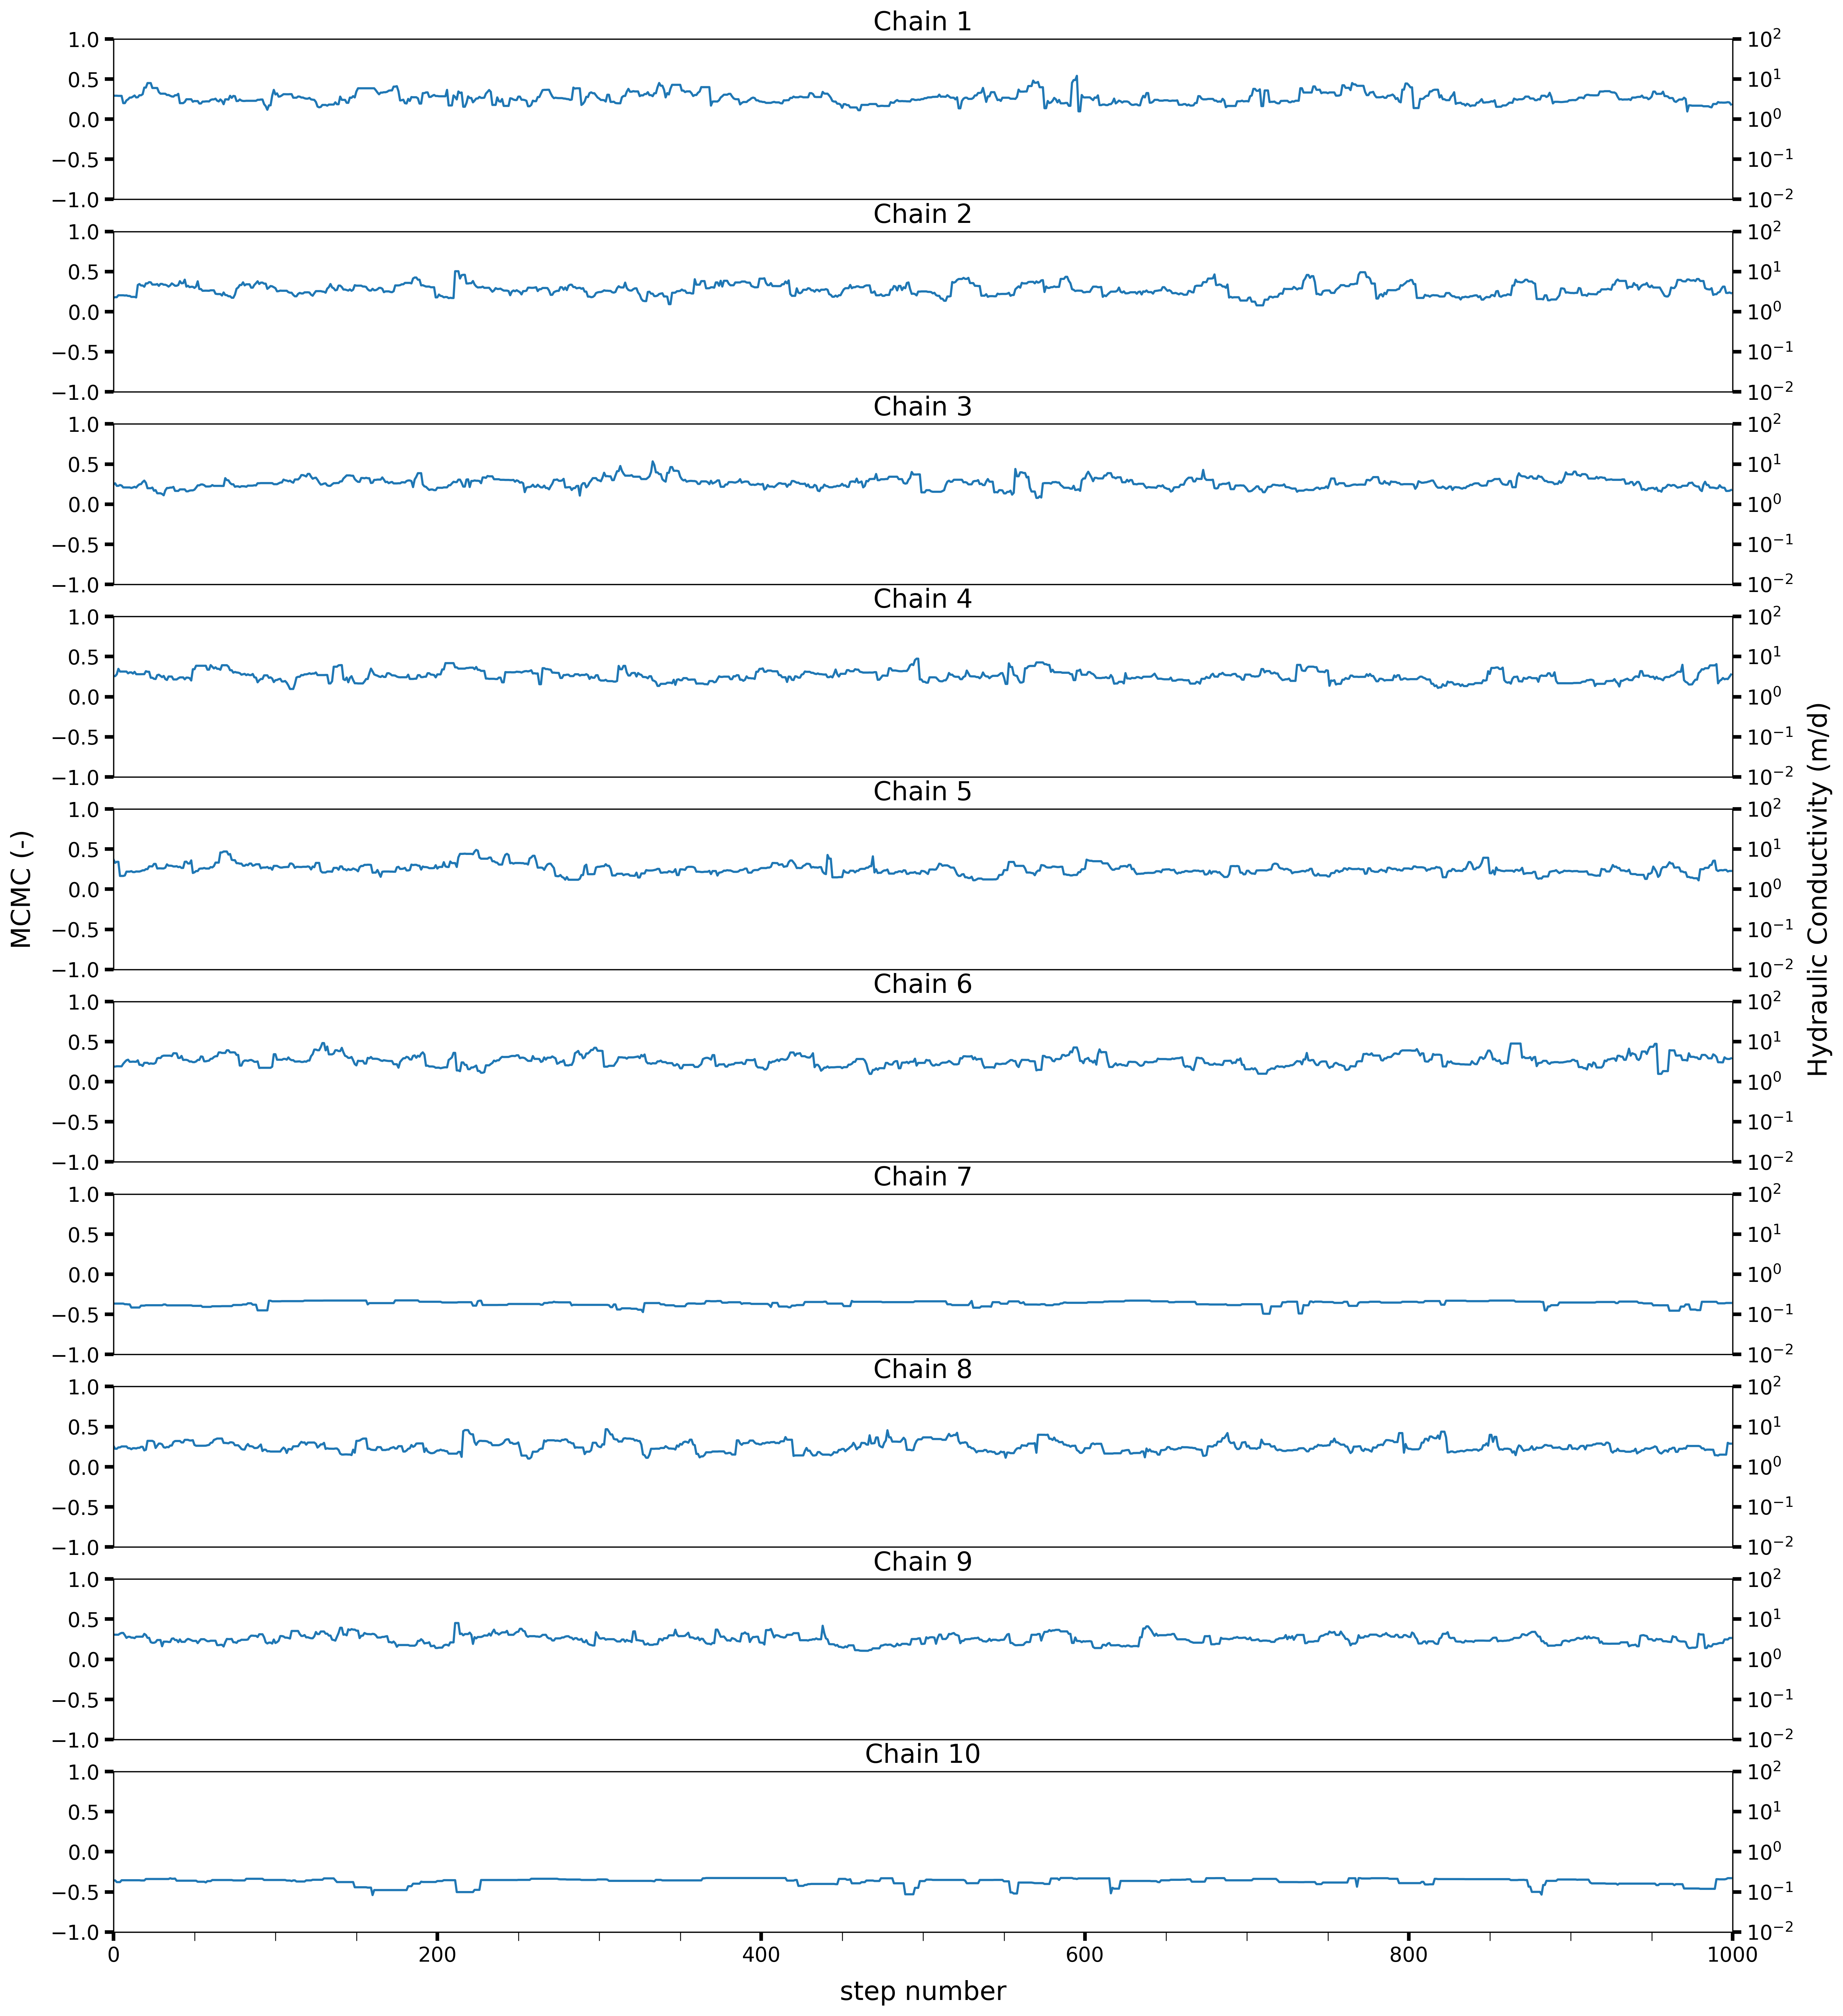
\includegraphics[width=1.0\textwidth]{Figures/appendix_figs/trace_plots_ensemble2_Stretch priornarrow.png}
\caption{Trace plots for ensemble 2 of AI from calibrating  $\theta_1$ in Model 1 with the narrow prior and 5 observations. All post burn-in steps are shown for all 10 chains, with the step number given on the x-axis. On the left y-axis the parameter values as used by the MCMC algorithm are shown. And on the right y-axis the transformed parameter values, used by MODFLOW 6, for calculation of the likelihood. For this ensemble $\hat{R}=1.44$.}\label{traceplot_AI_priornarrow}
\end{figure*}

\FloatBarrier
\subsubsection{DE}\label{sub_DE}
\begin{figure*}[ht]
\centering
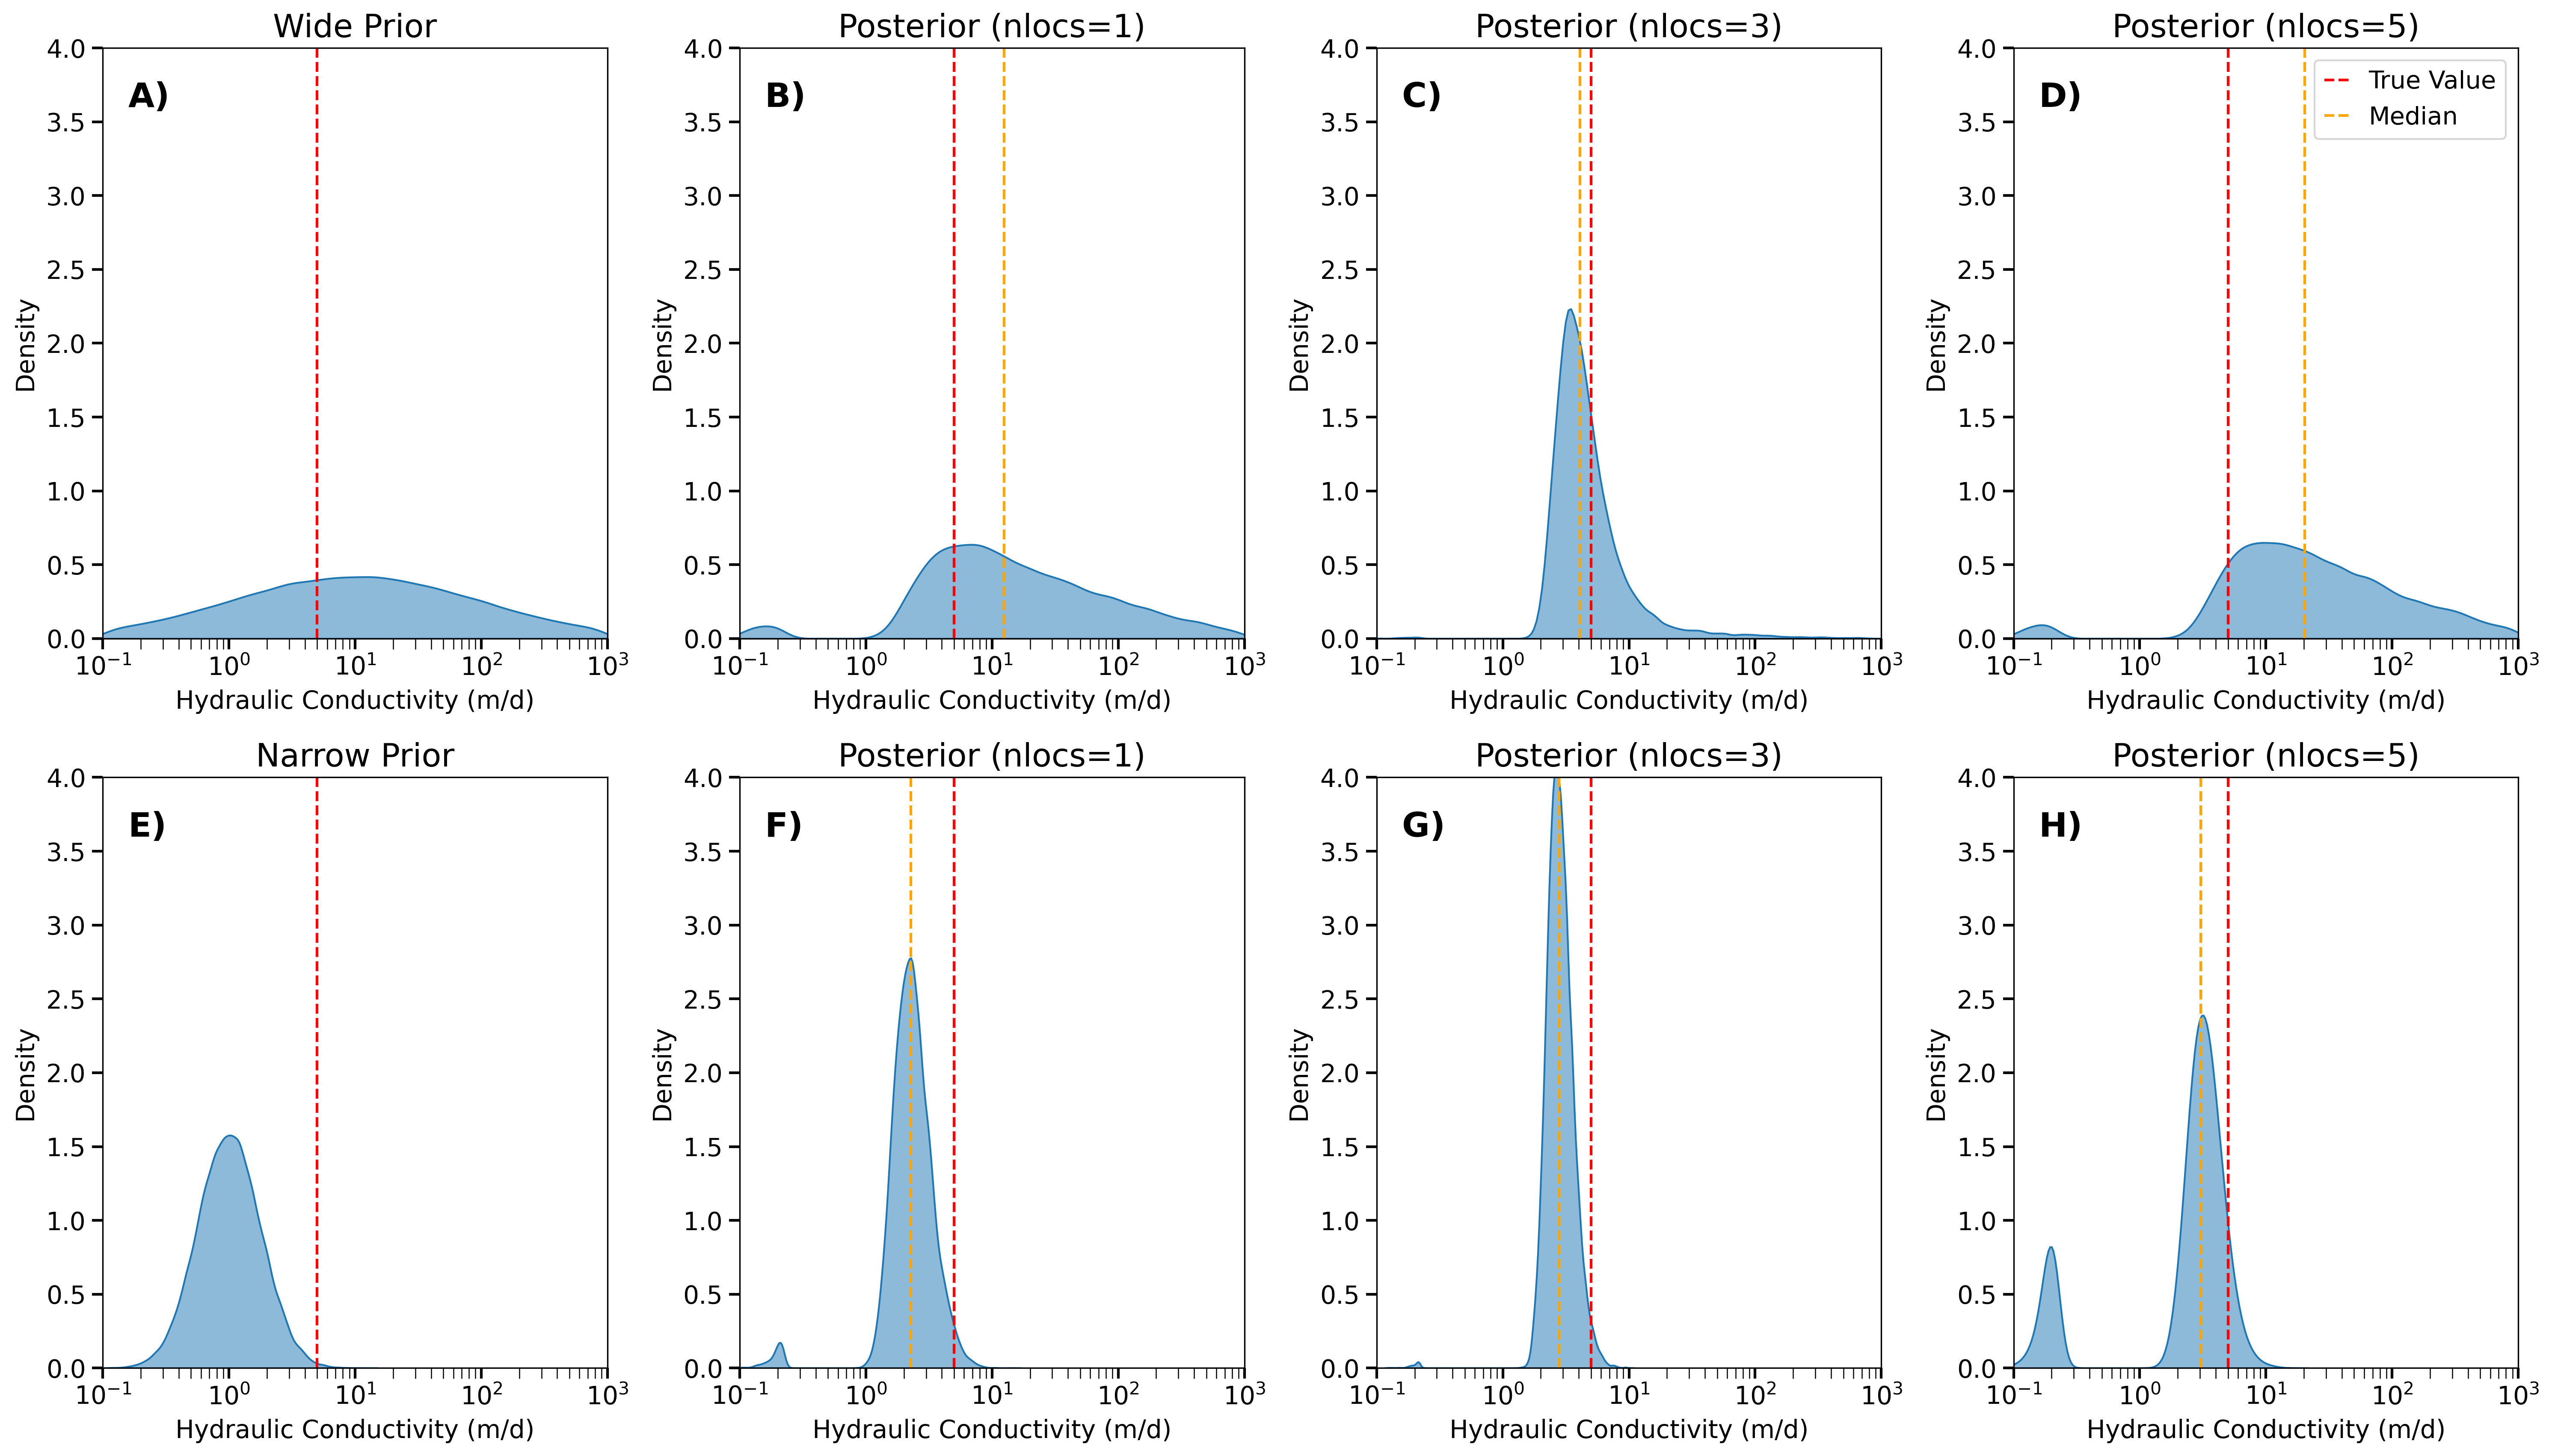
\includegraphics[width=1.0\textwidth]{Figures/appendix_figs/kde_model1_DE.png}
\caption{Kernel Density Estimate plots for the only parameter of Model 1 \textbf{($\theta_1$)}, which was calibrated with DE. \textbf{A)} shows the uninformative prior. \textbf{B), C)} and \textbf{D)} show the posteriors after calibrating $\theta_1$ with: the uninformative prior in combination with 1,3 or 5 observations for evaluating the likelihood. Similarly, \textbf{E)} shows the informative prior. \textbf{F), G)} and \textbf{H)} show the posteriors after calibrating $\theta_1$ with: the informative prior in combination with 1,3 or 5 observations for evaluating the likelihood. In each plot the dashed red line indicates the true value for $\theta_1$). Similarly, the posterior median is indicated by a dashed yellow line.}\label{fig_kde_model1_DE}
\end{figure*}

\begin{figure*}[ht]
\centering
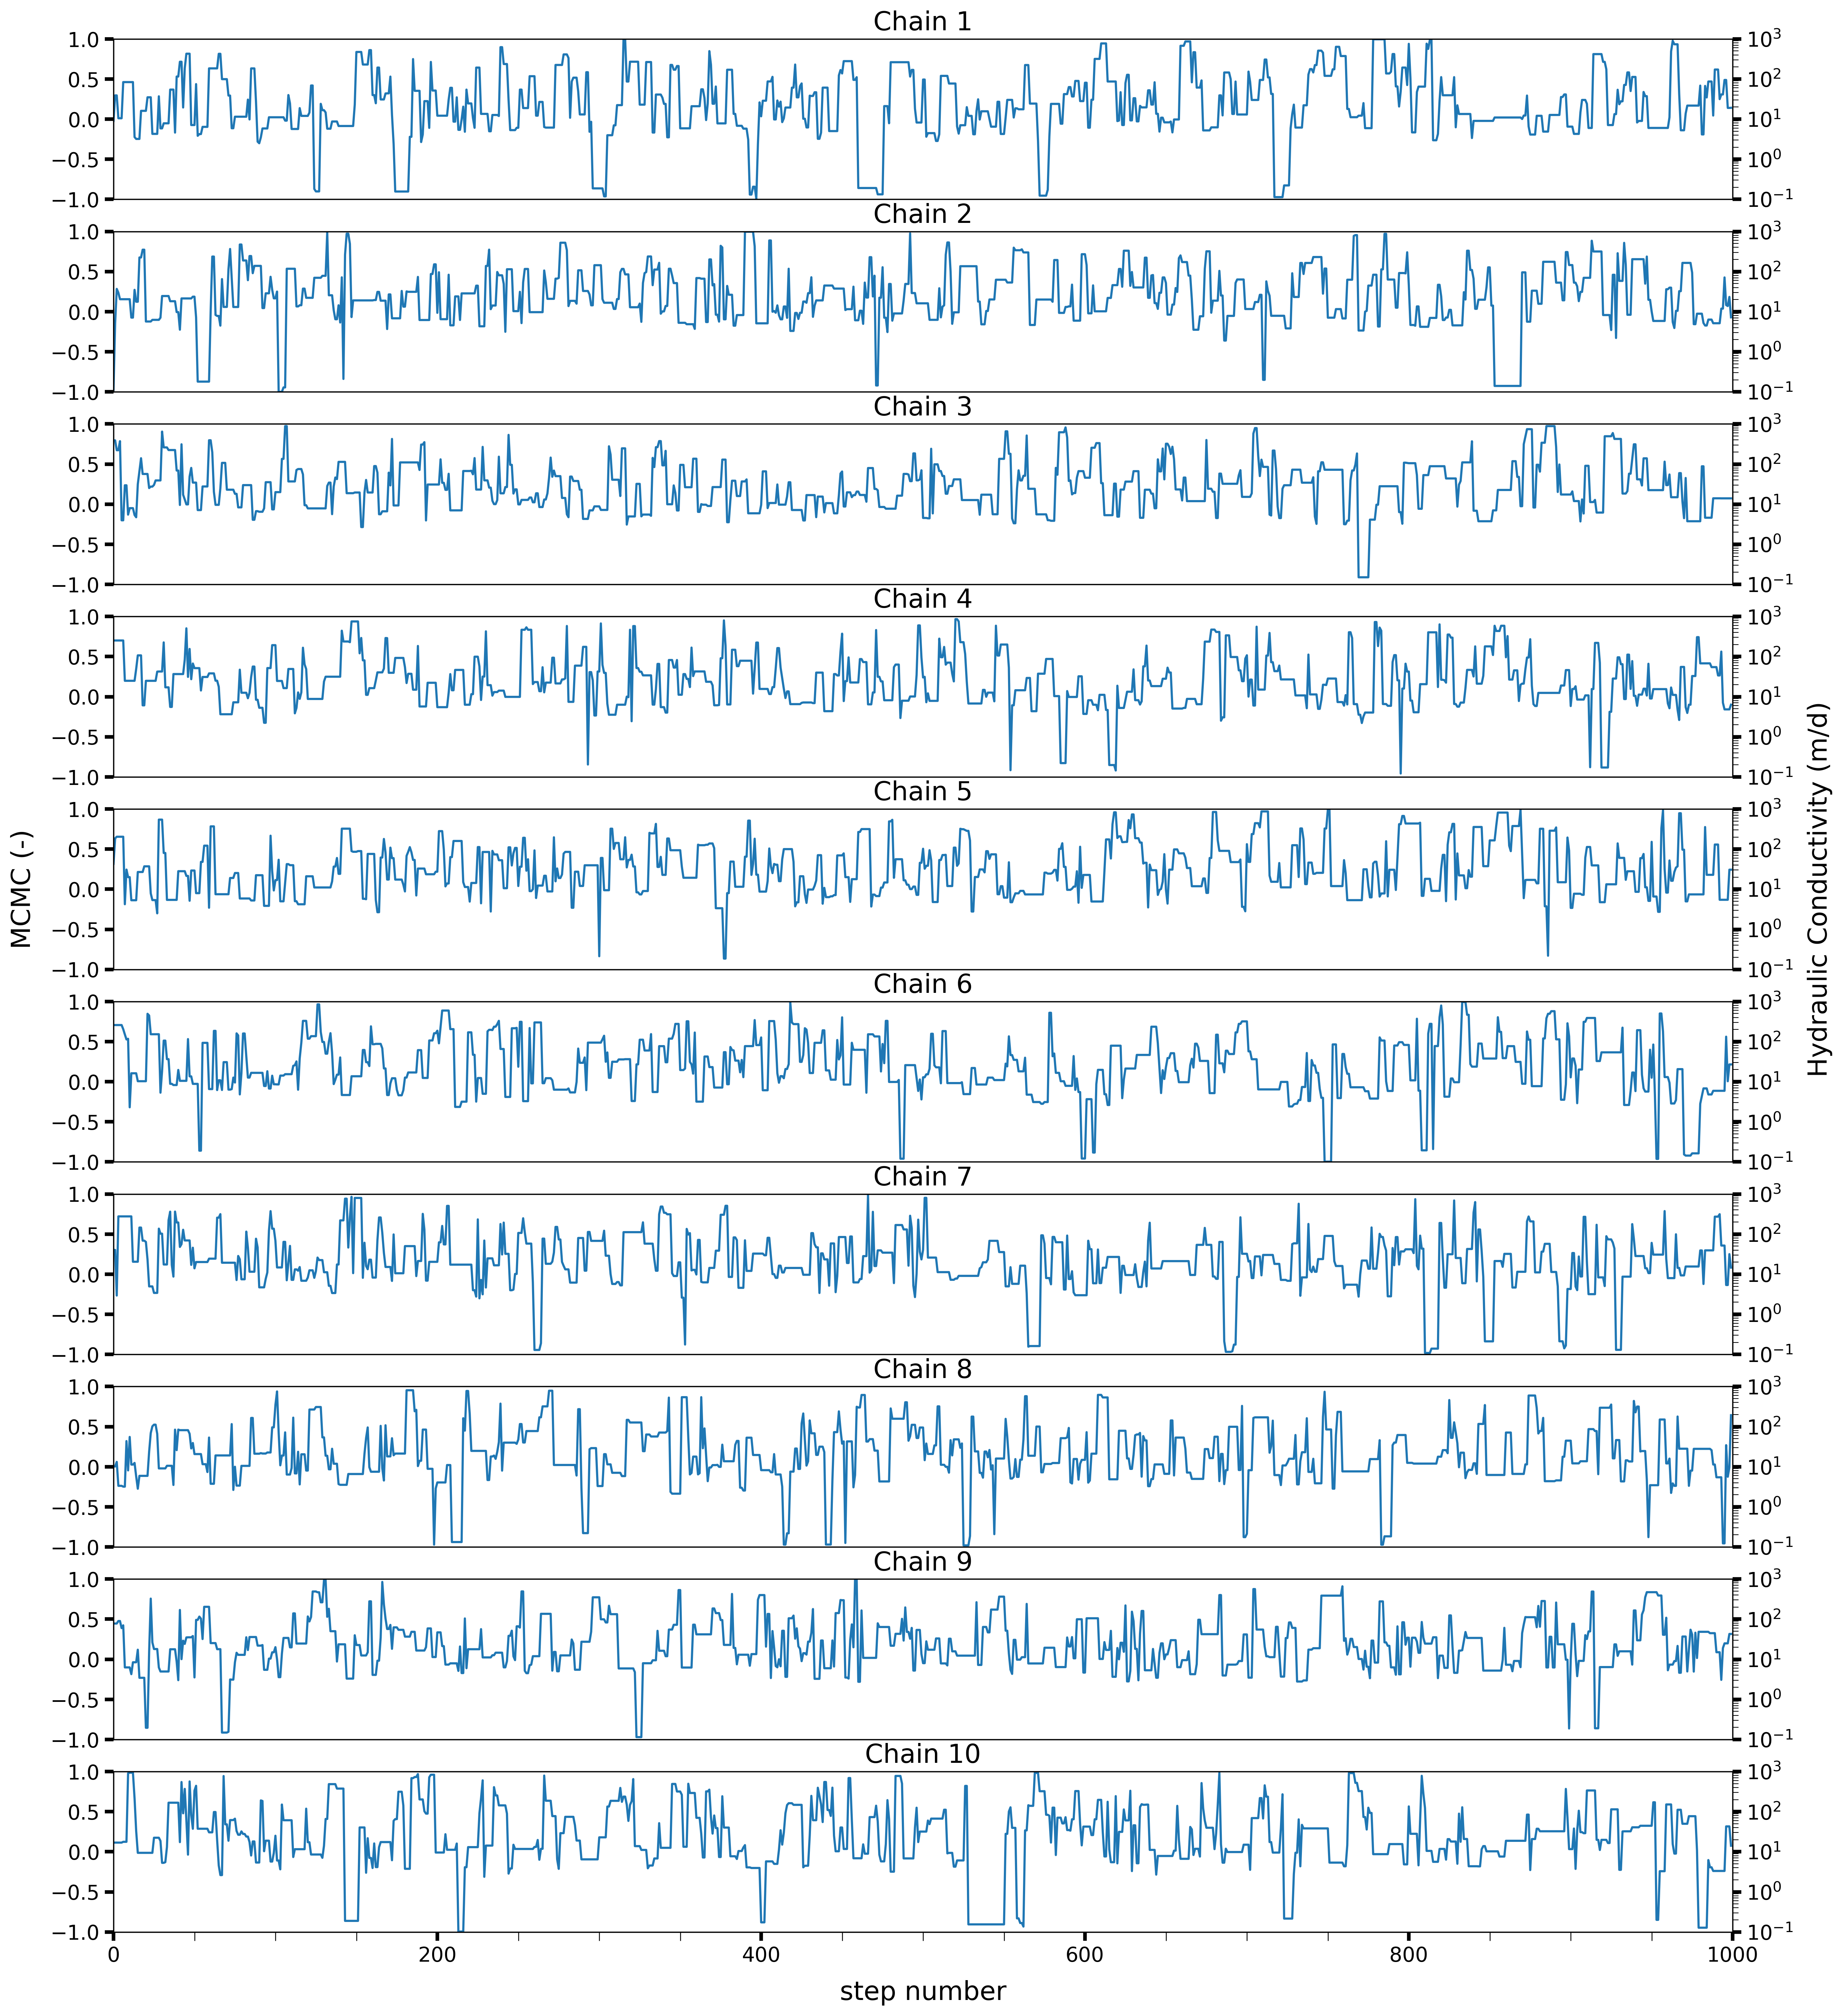
\includegraphics[width=1.0\textwidth]{Figures/appendix_figs/trace_plots_ensemble1_DE priorbroad.png}
\caption{Trace plots for ensemble 1 of DE from calibrating  $\theta_1$ in Model 1 with the wide prior and 5 observations. All post burn-in steps are shown for all 10 chains, with the step number given on the x-axis. On the left y-axis the parameter values as used by the MCMC algorithm are shown. And on the right y-axis the transformed parameter values, used by MODFLOW 6, for calculation of the likelihood. For this ensemble $\hat{R}=1.01$.}\label{traceplot_DE_priorbroad}
\end{figure*}

\begin{figure*}[ht]
\centering
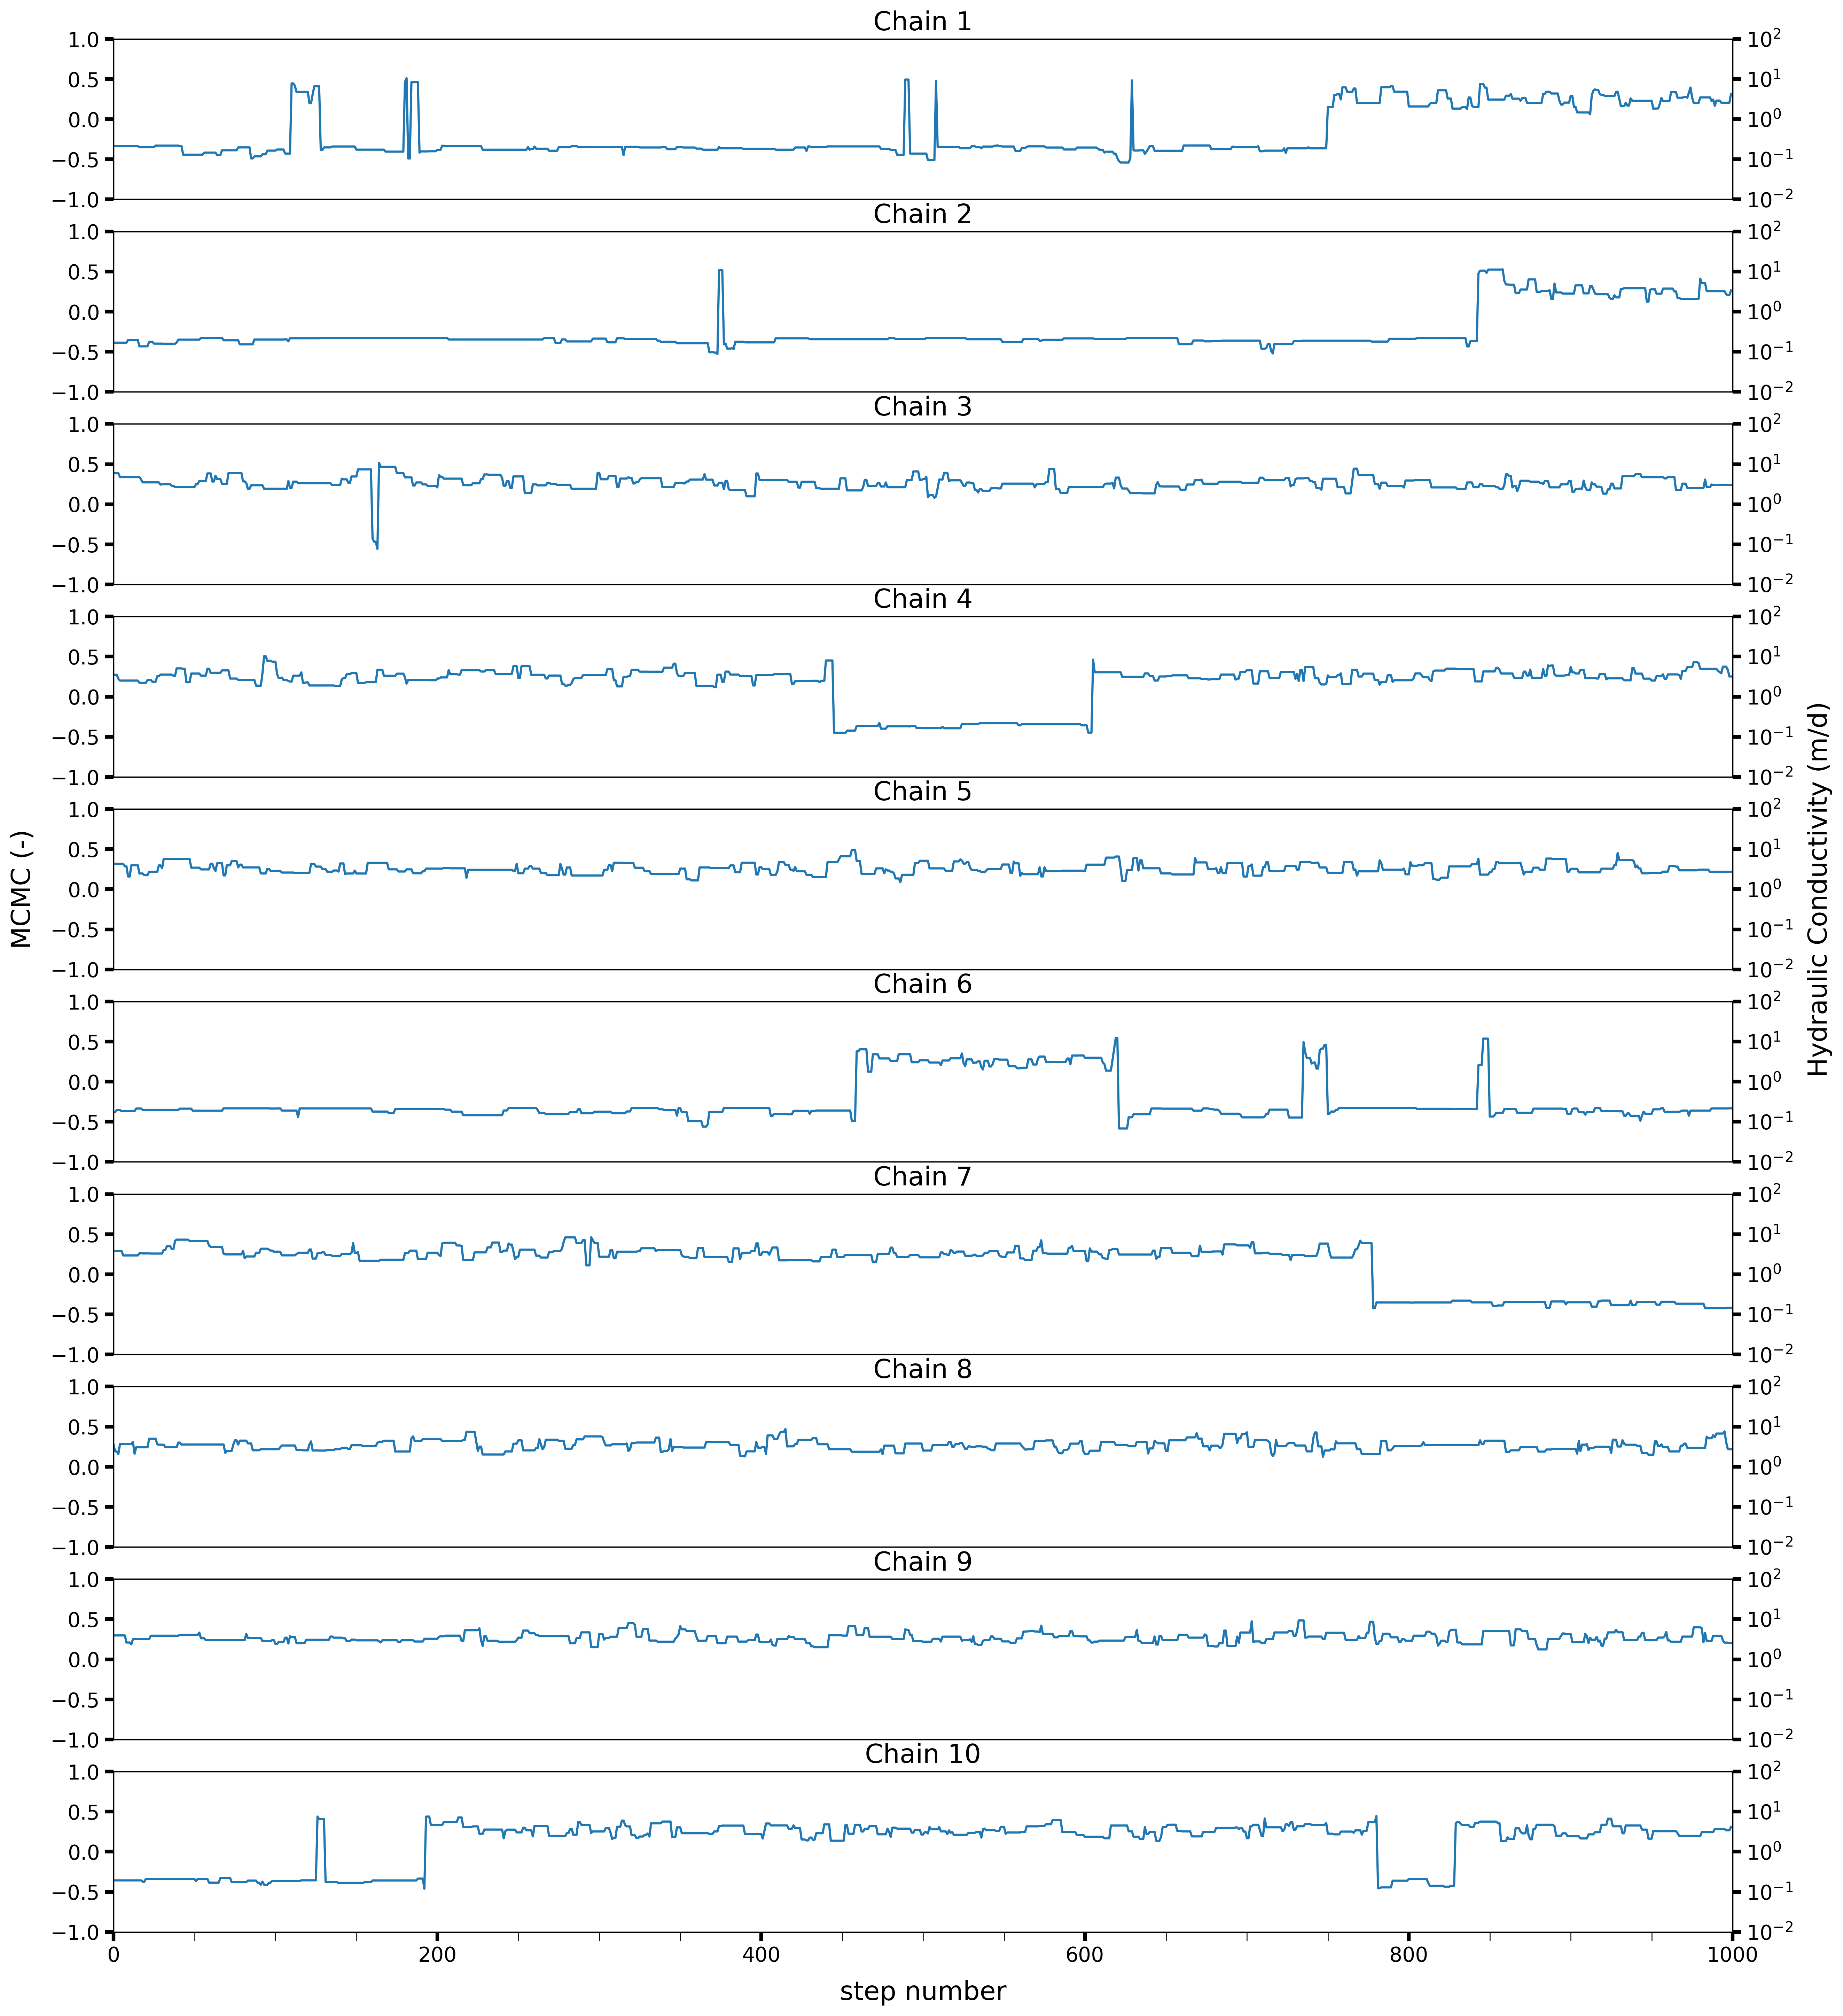
\includegraphics[width=1.0\textwidth]{Figures/appendix_figs/trace_plots_ensemble5_DE priornarrow.png}
\caption{Trace plots for ensemble 5 of DE from calibrating  $\theta_1$ in Model 1 with the narrow prior and 5 observations. All post burn-in steps are shown for all 10 chains, with the step number given on the x-axis. On the left y-axis the parameter values as used by the MCMC algorithm are shown. And on the right y-axis the transformed parameter values, used by MODFLOW 6, for calculation of the likelihood. For this ensemble $\hat{R}=1.27$.}\label{traceplot_DE_priornarrow}
\end{figure*}

\FloatBarrier
\subsubsection{DE-SNK}\label{sub_DE-SNK}
\begin{figure*}[ht]
\centering
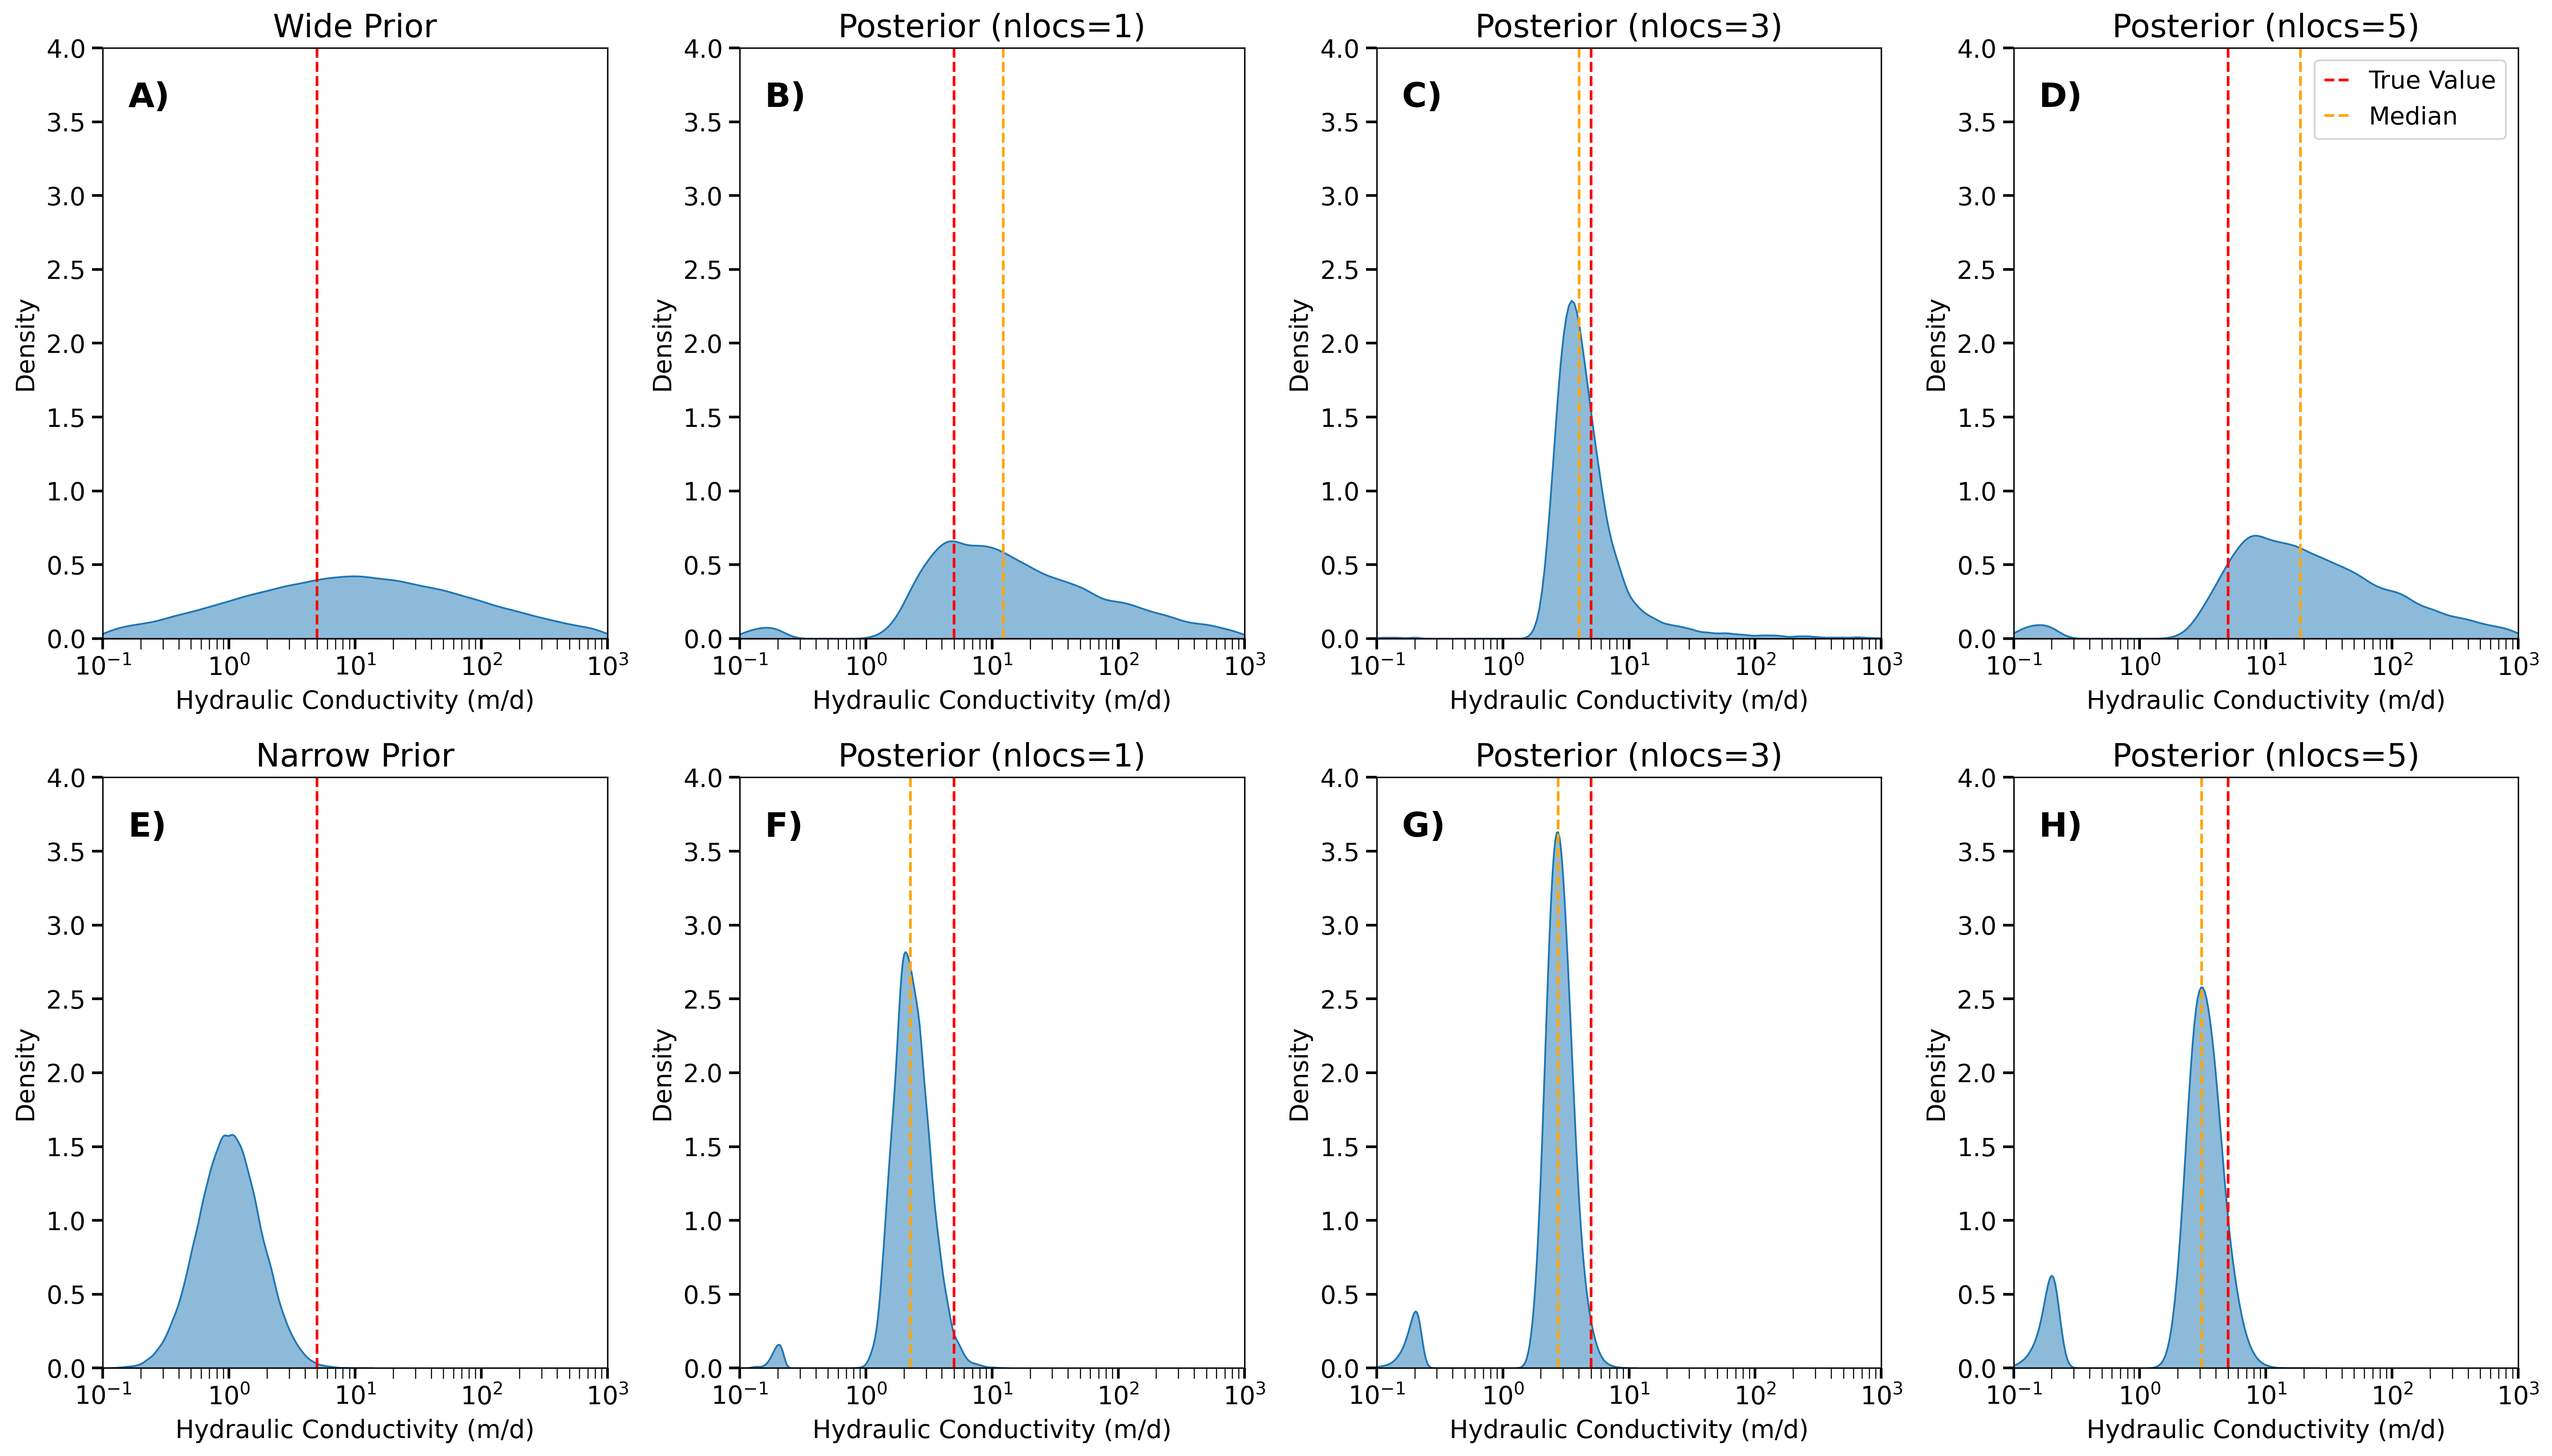
\includegraphics[width=1.0\textwidth]{Figures/kde_model1_DEsnooker.png}
\caption{Kernel Density Estimate plots for the only parameter of Model 1 ($\theta_1$), which was calibrated with DE-SNK. \textbf{A)} shows the wide prior. \textbf{B), C)} and \textbf{D)} show the posteriors after calibrating $\theta_1$ with: the wide prior in combination with 1,3 or 5 observations for evaluating the likelihood, respectively. Similarly, \textbf{E)} shows the narrow prior. \textbf{F), G)} and \textbf{H)} show the posteriors after calibrating $\theta_1$ with: the narrow prior in combination with 1,3 or 5 observations for evaluating the likelihood. In each plot the dashed red line indicates the true value for $\theta_1$. Similarly, the posterior median is indicated by a dashed yellow line.}\label{fig_kde_model1_DEsnooker_app}
\end{figure*}

\begin{figure*}[ht]
\centering
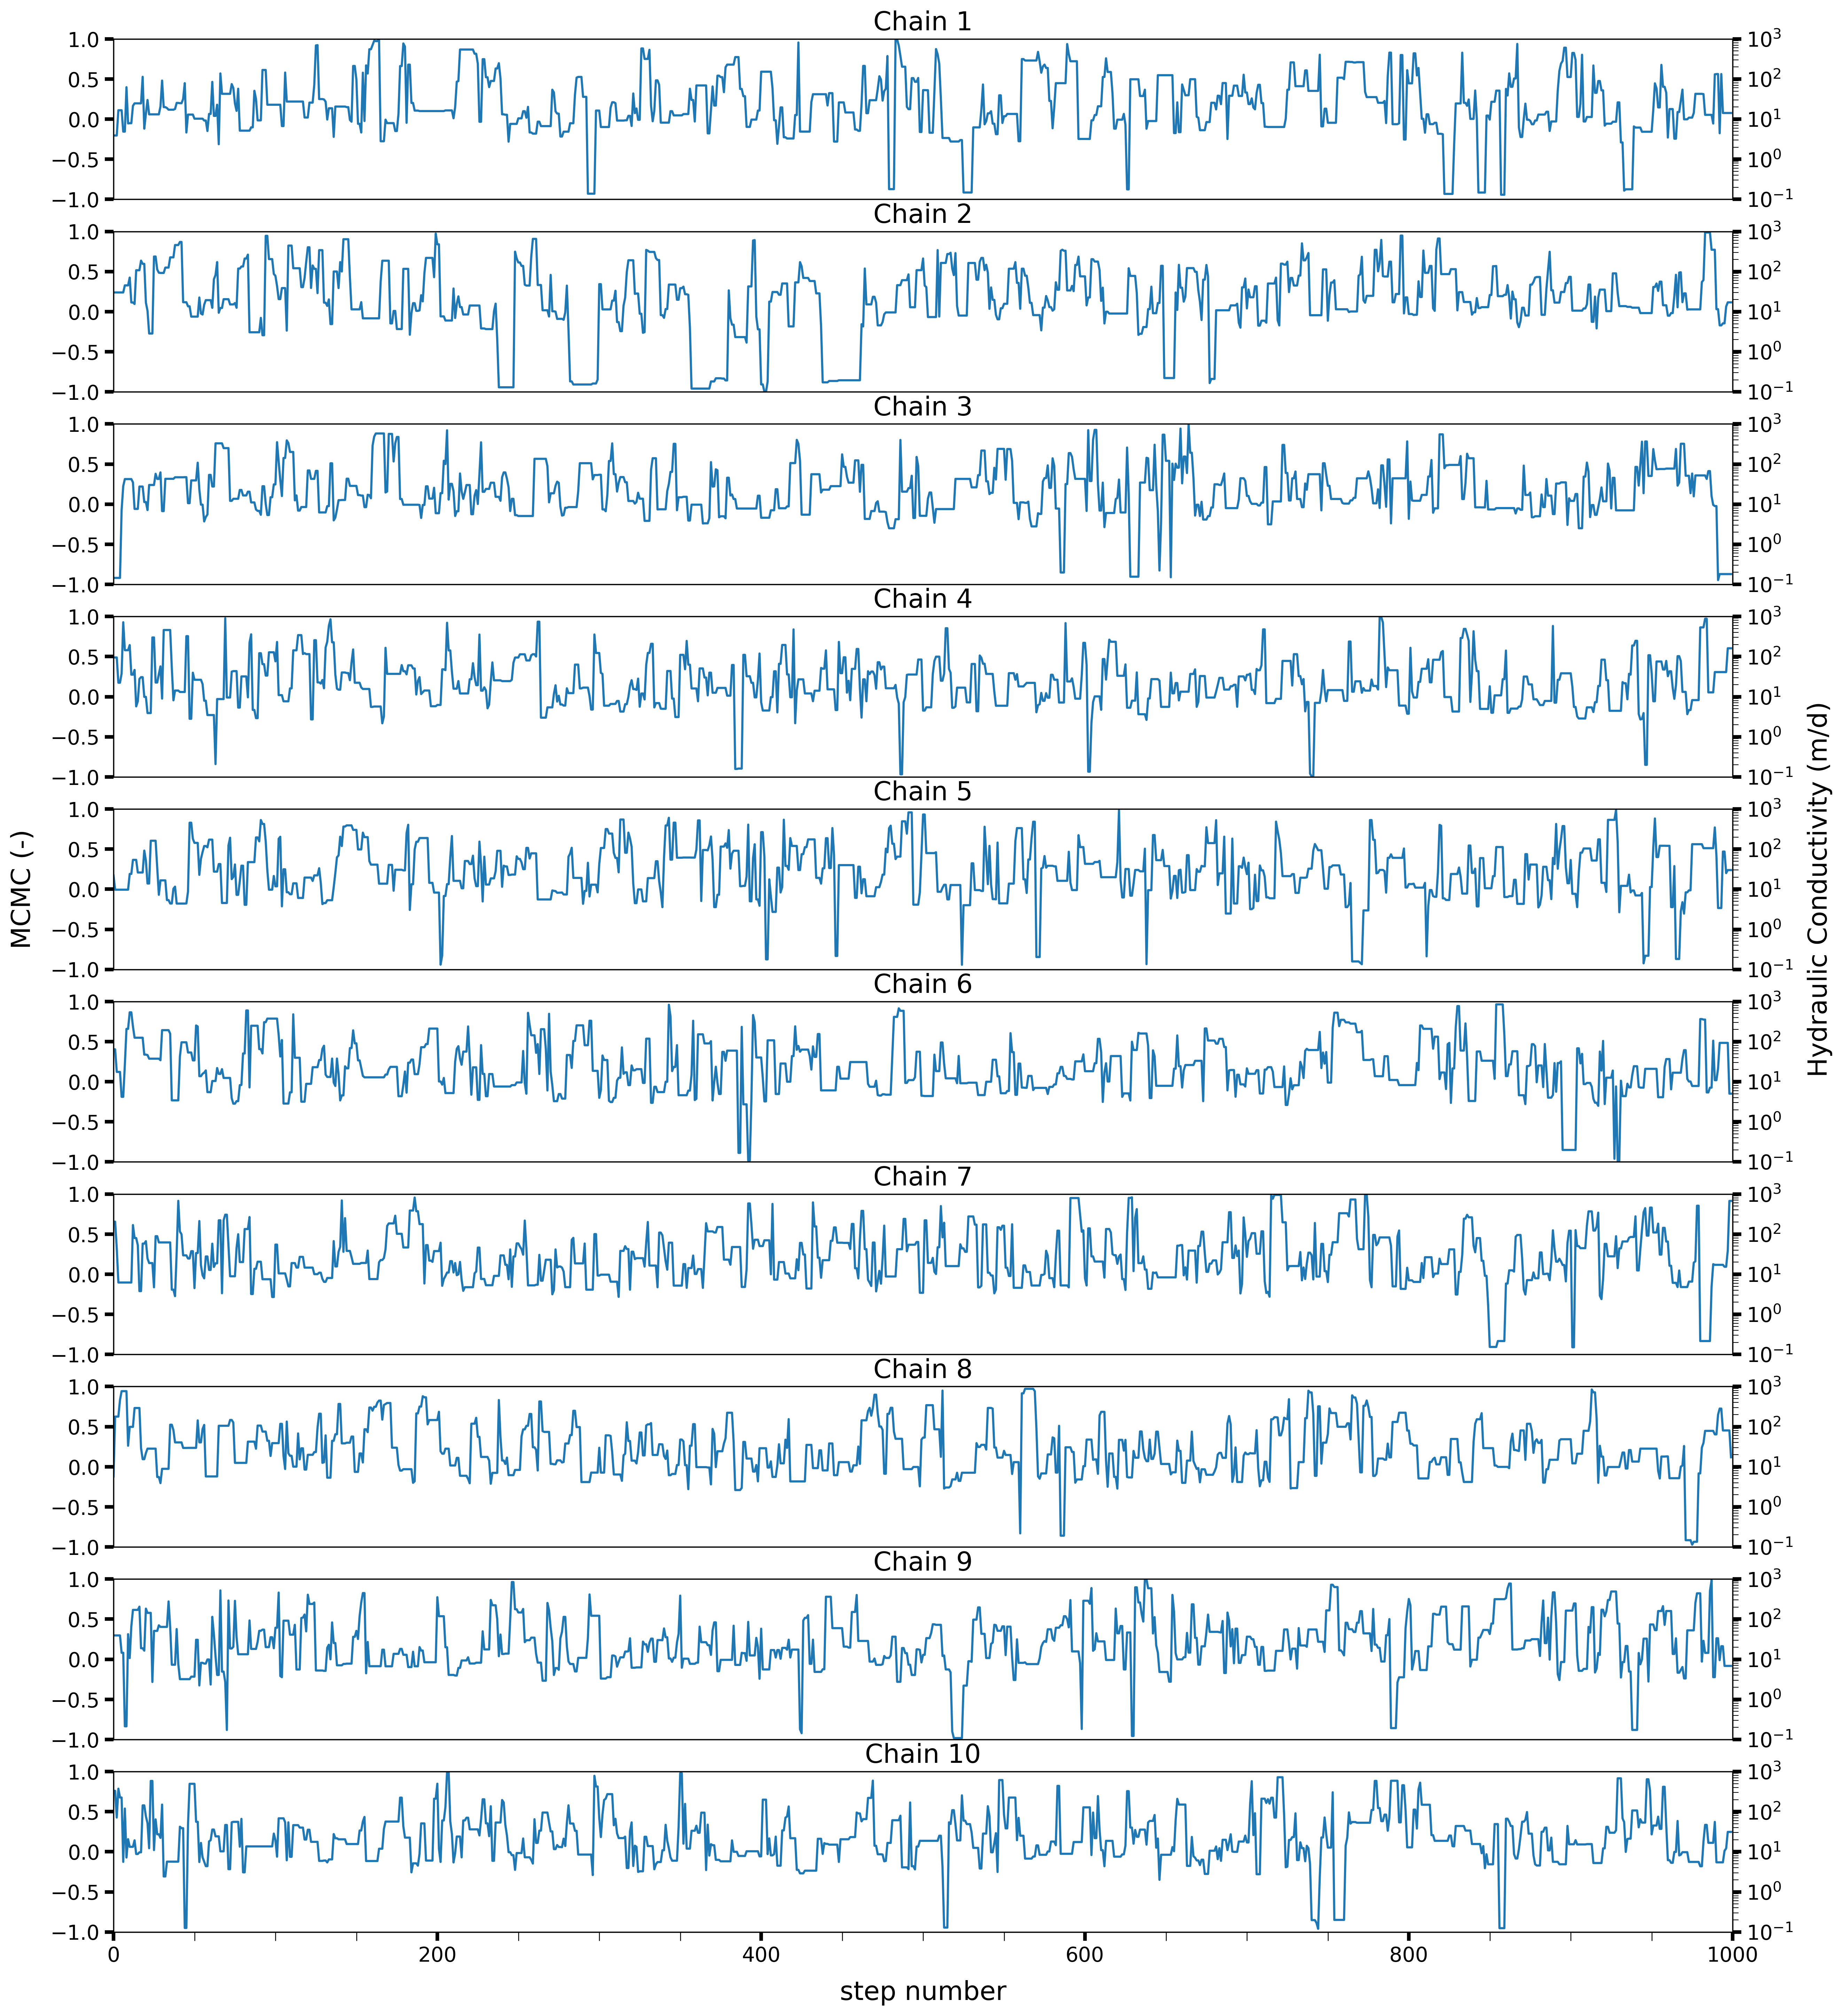
\includegraphics[width=1.0\textwidth]{Figures/appendix_figs/trace_plots_ensemble4_DEsnooker priorbroad.png}
\caption{Trace plots for ensemble 4 of DE-SNK from calibrating  $\theta_1$ in Model 1 with the wide prior and 5 observations. All post burn-in steps are shown for all 10 chains, with the step number given on the x-axis. On the left y-axis the parameter values as used by the MCMC algorithm are shown. And on the right y-axis the transformed parameter values, used by MODFLOW 6, for calculation of the likelihood. For this ensemble $\hat{R}=1.01$.}\label{traceplot_DE-SNK_priorbroad}
\end{figure*}

\begin{figure*}[ht]
\centering
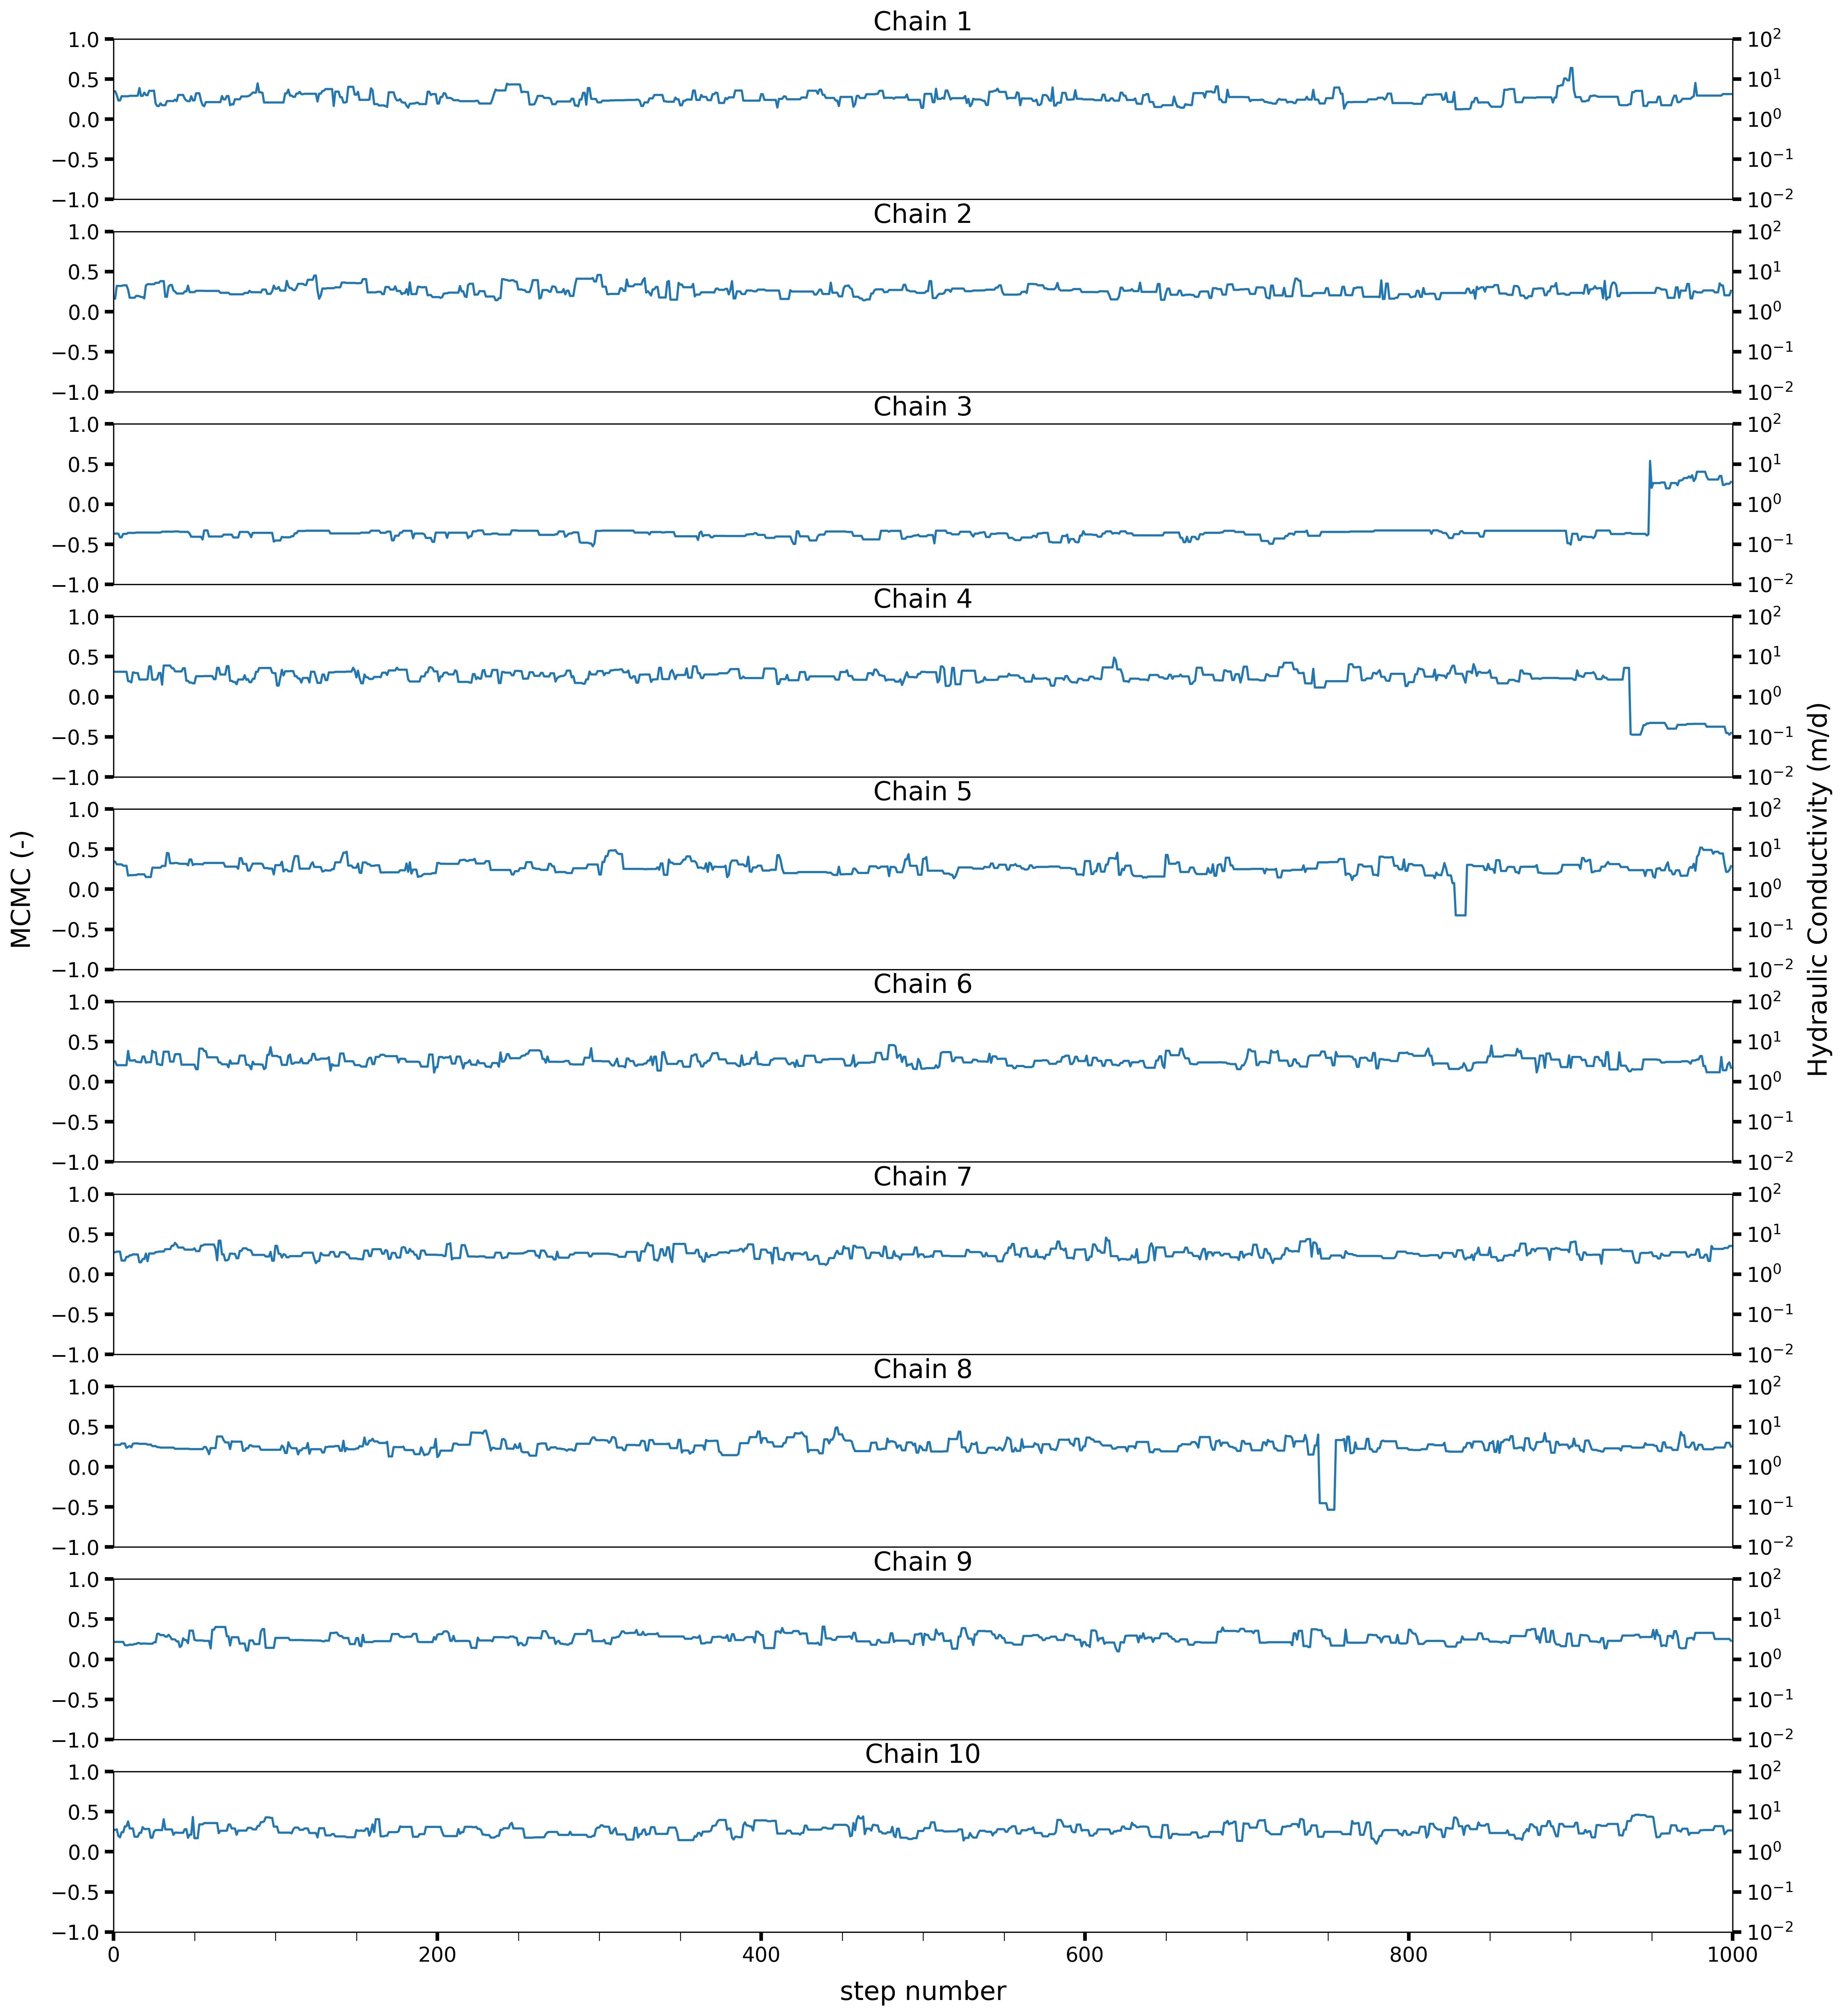
\includegraphics[width=1.0\textwidth]{Figures/appendix_figs/trace_plots_ensemble3_DEsnooker priornarrow.png}
\caption{Trace plots for ensemble 3 of DE-SNK from calibrating  $\theta_1$ in Model 1 with the narrow prior and 5 observations. All post burn-in steps are shown for all 10 chains, with the step number given on the x-axis. On the left y-axis the parameter values as used by the MCMC algorithm are shown. And on the right y-axis the transformed parameter values, used by MODFLOW 6, for calculation of the likelihood. For this ensemble $\hat{R}=1.21$.}\label{traceplot_DE-SNK_priornarrow}
\end{figure*}


